% This is the Duke University Statistical Science LaTeX thesis template.
% It has been adapted from the Reed College LaTeX thesis template. The
% adaptation was done by Mine Cetinkaya-Rundel (MCR). Some of the comments
% that are specific to Reed College have been removed.
%
% Most of the work on the original Reed College document class and template
% was done by Sam Noble (SN). Later comments etc. by Ben Salzberg (BTS).
% Additional restructuring and APA support by Jess Youngberg (JY).
%
% See https://www.reed.edu/cis/help/latex/ for help. There are a
% great bunch of help pages there, with notes on
% getting started, bibtex, etc. Go there and read it if you're not
% already familiar with LaTeX.
%
% Any line that starts with a percent symbol is a comment.
% They won't show up in the document, and are useful for notes
% to yourself and explaining commands.
% Commenting also removes a line from the document;
% very handy for troubleshooting problems. -BTS

%%
%% Preamble
%%
% \documentclass{<something>} must begin each LaTeX document
\documentclass[12pt,twoside]{dukestatscithesis}
% Packages are extensions to the basic LaTeX functions. Whatever you
% want to typeset, there is probably a package out there for it.
% Chemistry (chemtex), screenplays, you name it.
% Check out CTAN to see: http://www.ctan.org/
%%
\usepackage{graphicx,latexsym}
\usepackage{amsmath}
\usepackage{amssymb,amsthm}
\usepackage{longtable,booktabs,setspace}
\usepackage{chemarr} %% Useful for one reaction arrow, useless if you're not a chem major
\usepackage[hyphens]{url}
% Added by CII
\usepackage{hyperref}
\usepackage{lmodern}
\usepackage{float}
\floatplacement{figure}{H}
% End of CII addition
\usepackage{rotating}

% Next line commented out by CII
%%% \usepackage{natbib}
% Comment out the natbib line above and uncomment the following two lines to use the new
% biblatex-chicago style, for Chicago A. Also make some changes at the end where the
% bibliography is included.
%\usepackage{biblatex-chicago}
%\bibliography{thesis}


% Added by CII (Thanks, Hadley!)
% Use ref for internal links
\renewcommand{\hyperref}[2][???]{\autoref{#1}}
\def\chapterautorefname{Chapter}
\def\sectionautorefname{Section}
\def\subsectionautorefname{Subsection}
% End of CII addition

% Added by CII
\usepackage{caption}
\captionsetup{width=5in}
% End of CII addition

% \usepackage{times} % other fonts are available like times, bookman, charter, palatino


% To pass between YAML and LaTeX the dollar signs are added by CII
\title{}
\author{}
% The month and year that you submit your FINAL draft TO THE LIBRARY (May or December)
\date{}
\advisor{}
\institution{}
\degree{}
\committeememberone{}
\committeemembertwo{}
\dus{}
%If you have two advisors for some reason, you can use the following
% Uncommented out by CII
% End of CII addition

%%% Remember to use the correct department!
\department{}

% Added by CII
%%% Copied from knitr
%% maxwidth is the original width if it's less than linewidth
%% otherwise use linewidth (to make sure the graphics do not exceed the margin)
\makeatletter
\def\maxwidth{ %
  \ifdim\Gin@nat@width>\linewidth
    \linewidth
  \else
    \Gin@nat@width
  \fi
}
\makeatother

\renewcommand{\contentsname}{Table of Contents}
% End of CII addition

\setlength{\parskip}{0pt}

% Added by CII

\providecommand{\tightlist}{%
  \setlength{\itemsep}{0pt}\setlength{\parskip}{0pt}}

\Acknowledgements{

}

\Dedication{

}

\Preface{

}

\Abstract{

}

% End of CII addition
%%
%% End Preamble
%%
%

\usepackage{amsthm}
\newtheorem{theorem}{Theorem}[chapter]
\newtheorem{lemma}{Lemma}[chapter]
\theoremstyle{definition}
\newtheorem{definition}{Definition}[chapter]
\newtheorem{corollary}{Corollary}[chapter]
\newtheorem{proposition}{Proposition}[chapter]
\theoremstyle{definition}
\newtheorem{example}{Example}[chapter]
\theoremstyle{definition}
\newtheorem{exercise}{Exercise}[chapter]
\theoremstyle{remark}
\newtheorem*{remark}{Remark}
\newtheorem*{solution}{Solution}
\begin{document}

% Everything below added by CII

\frontmatter % this stuff will be roman-numbered
\pagestyle{empty} % this removes page numbers from the frontmatter



  \hypersetup{linkcolor=black}
  \setcounter{tocdepth}{2}
  \tableofcontents





\mainmatter % here the regular arabic numbering starts
\pagestyle{fancyplain} % turns page numbering back on

\chapter{Introduction}\label{intro}

Sentiment analysis, the study of complex human affections and subjective
information, is a special focus in text mining and natural language
processing. With the widespread use of social media in the digital age,
sentiment analysis has become an increasingly useful tool for opinion
mining and monitoring in different field. Among its many applications,
the extraction of sentiments and opinions in user-generated reviews such
as reviews of products, movies, or restaurants has engaged much interest
given its representation of a direct ``voice'' of customers and the
value embedded in and beneath the words themselves.

While analyses of these voice-of-the-customer (VOC) materials mainly
focus on the classification of sentiment polarity at the document level,
reviews rarely embodies a single sentiment towards a particular object
or entity, but often times involve complex, multi-level, and sometimes
contradicting sentiments towards multiple aspects of the same entity.
For example, a restaurant review may have an overall positive sentiment
towards the experience as a whole, but more specifically a particularly
positive sentiment towards the service, neutral towards ambience, and
even negative towards the food. These common aspects and their
associated sentiments are key to understanding the review and the
reviewed entity and can be of great use in many application cases
including personalization.

This report proposes a potential procedure for extracting such common
topics using topic modeling, illustrated with the Yelp dataset of
restaurant reviews. Next steps regarding the aggregation of sentiments
associated with these topics will also be discussed.

\chapter{Methodology}\label{methods}

\section{Data Preprocessing}\label{data-preprocessing}

Standard text data cleaning procedure was followed for the preprocessing
of the review corpus: all characters were transformed to lowercase,
punctuations and numbers were removed, stop words such as ``I'', ``me'',
``she'', ``is'' (see Appendix: stopwords for the full list) were also
removed, whitespaces were stripped and trimmed, and all words were
stemmed using Porter stemming algorithm (implemented in R through the
stemDocument function in the tm package).

\section{N-Gramming}\label{n-gramming}

One optional yet particularly helpful preprocessing step was n-gramming.
It captures word sequences that are better perceived or carry more
meaningful information as a whole. For example, ``White House'' should
be perceived as a single token instead of separately as ``white'' and
``house'', and similarly ``President of the United States'' makes more
sense as a whole. N-gramming is especially helpful when identifying word
sequences that are specific to the context of the corpus. In the
previous example, it would be crucial to identify ``White House'' and
``President of the United States'' as n-grams in a corpus consists of
political blogs. In our case where we have a corpus of restaurant
reviews, we can expect to see context-specific n-grams such as ``Mac `n
Cheese'', ``highly recommend'', ``great service'', and even ``can't wait
to go back''.

We adopted the probabilistic approach for identifying these n-grams
where the conditional probability of seeing the ith word given the
(i-1)th word. The n-gramming implementation code was modified based on
the NGramming Processing Script (c) by Teague Henry. The procedure in
this code is for each consecutive bigram sequence (word1, word2):
\begin{enumerate}
\def\labelenumi{\arabic{enumi}.}
\tightlist
\item
  Calculate count1 = number of appearances of word1 in the corpus;\\
\item
  Calculate prop2 = appearance rate of word2 in all non-word1 words in
  the corpus;\\
\item
  Calculate count\_bi = number of appearance of bigram word1\_word2 in
  the corpus;\\
\item
  Compute p\_value = Pr(N count\_bi) where N is the total number of
  consecutive co-occurrences of word1\_word2, N \textasciitilde{}
  Binomial(count1, prop2);\\
\item
  If p-value \textless{} 0.01, then we reject the null hypothesis that
  the co-occurrences happened by random and identify word1\_word2 as a
  meaningful bigram.
\end{enumerate}
The above procedure is repeated again after first run to identify
trigrams and larger n-grams.

In terms of the cutoff threshold for identifying meaningful n-grams,
both count and p-values were considered. While p-value cutoff has
comparatively more consistent performance, it alone would include
bigrams with neglectable occurrences (eg. appeared only 2 times in the
entire corpus) and thus contribute minimal information. As a result, a
hybrid cutoff using both a p-value cutoff of 0.01 and empirically-set
count cutoffs of 100 for bigrams and 40 for trigrams was adopted for our
corpus.

All identified n-grams will be replaced by an integrated token of the
original words in the corpus, where bigrams are connected with ``\_'' in
between and trigrams with ``.''. For example, after all pre-processing
steps and n-gramming, ``White House'' would become ``white\_hous'', and
``Mac `n Cheese'' would be ``mac\_n.chees.''

\section{Topic Extraction}\label{topic-extraction}

\subsection{Latent Dirichlet Allocation
(LDA)}\label{latent-dirichlet-allocation-lda}

To identify common topics in our corpus, we will first experiment with
the topic modeling approach, or more specifically Latent Dirichlet
Allocation (LDA). LDA is a Bayesian generative topic model based on the
assumption that each document, as a collection of words, is a mixture of
a certain number of topics, and that the occurrence of each word in that
document can be attributed to one of its topics. In terms of
denotations, the entire corpus is a set of documents
\(\{D_1, ..., Dm\}\), and the words within a document are denoted as
\(D_i=\{w_{i1},...,w_{in_i}\}\), \(w_ij \in W\) where W is a finite
vocabulary set of size \(V\). Suppose we assume the entire corpus is a
mixture of \(K\) topics, the data generative process with LDA is as
follows:
\begin{enumerate}
\def\labelenumi{\arabic{enumi}.}
\tightlist
\item
  For each topic \(k \in \{1,...,K\}\),\\
\end{enumerate}
\begin{enumerate}
\def\labelenumi{\alph{enumi}.}
\tightlist
\item
  Draw a topic-word proportion vector
  \(\phi_k \sim Dirichlet(\alpha)\)\\
\end{enumerate}
\begin{enumerate}
\def\labelenumi{\arabic{enumi}.}
\setcounter{enumi}{1}
\tightlist
\item
  For each document \(D_i\),
\end{enumerate}
\begin{enumerate}
\def\labelenumi{\alph{enumi}.}
\tightlist
\item
  Draw a document-topic proportion vector
  \(\theta_i \sim Dirichlet(\beta)\)\\
\item
  For each word \(w_{ij}\),
  \begin{enumerate}
  \def\labelenumii{\roman{enumii}.}
  \tightlist
  \item
    Draw a topic assignment
    \(z_j \sim Multinomial(\theta_i), z_j \in \{1,...,K\}\)\\
  \item
    Draw a word from this topic
    \(w_{ij} \sim Multinomial(\phi_k), w_{ij} \in \{1,...,V\}\)
  \end{enumerate}
\end{enumerate}
\begin{figure}[htbp]
\centering
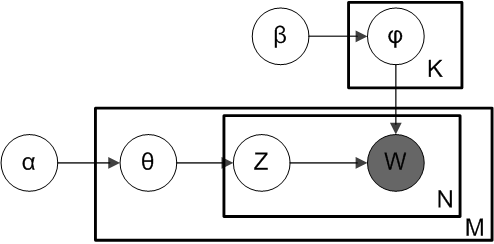
\includegraphics{figure/LDA.png}
\caption{\label{fig:LDA}LDA data generative process (Wikipedia)}
\end{figure}
For our corpus, currently the number of topics is manually set at 5, so
a future step would be determining the best number of topics for the
corpus.

\section{Sentiment Extraction and Aggregation (Spring
Semester)}\label{sentiment-extraction-and-aggregation-spring-semester}

\chapter{Results}\label{results}

The Yelp dataset version as of Round 10 (in terms of the Dataset
Challenge) contains 4.7 million reviews of 156K businesses, not limited
to restaurants and each with corresponding attributes such as business
hours, parking, and ambience. For the purpose of this thesis, we
restrict to reviews of restaurants in the US and only examine a sample
of this subset, which comes to 57,790 reviews of 1,409 restaurant in the
US provided by 47,617 users on Yelp.

\section{Exploratory Data Analysis}\label{exploratory-data-analysis}

Before diving into the analysis of the corpus, we shall first explore
the distribution and characteristics of the reviews and the reviewed
restaurants. Note that the insights here does not necessarily reflect
the actual distribution or characteristics of the reviewed restaurants
or reviews on Yelp since our corpus is a sample of the Yelp-provided
dataset which is also a not necessarily random sample of the raw
reviews.

As shown below in the graphs, 258 out of the 1409 restaurants reviewed
in our corpus are located in the state of Arizona, and the majority of
the reviewed restaurants also in Nevada, Ohio, North Carolina, and
Pennsylvania, with the rest of the restaurants in Wisconsin and Illinois
and only a few in South Carolina, California, or New York. The state
distribution may later explain the identification of certain
location-specific n-grams such as ``las\_vega.'' On average each
restaurant has 40 reviews in our corpus, with 50\% of them having around
10 reviews and 10\% having more than 100 reviews. The review-restaurant
distribution may influence the choice and validity of any potential
segmentation of the corpus for analysis or later the aggregation of
sentiments by restaurants. Most reviews in our corpus are relatively
short with an average length of 115 words (median at 81 words), while
there surely are more lengthy reviews, with about 3,500 reviews (6\% of
all reviews) spanning from 300 to 1,000 words.
\begin{figure}[htbp]
\centering
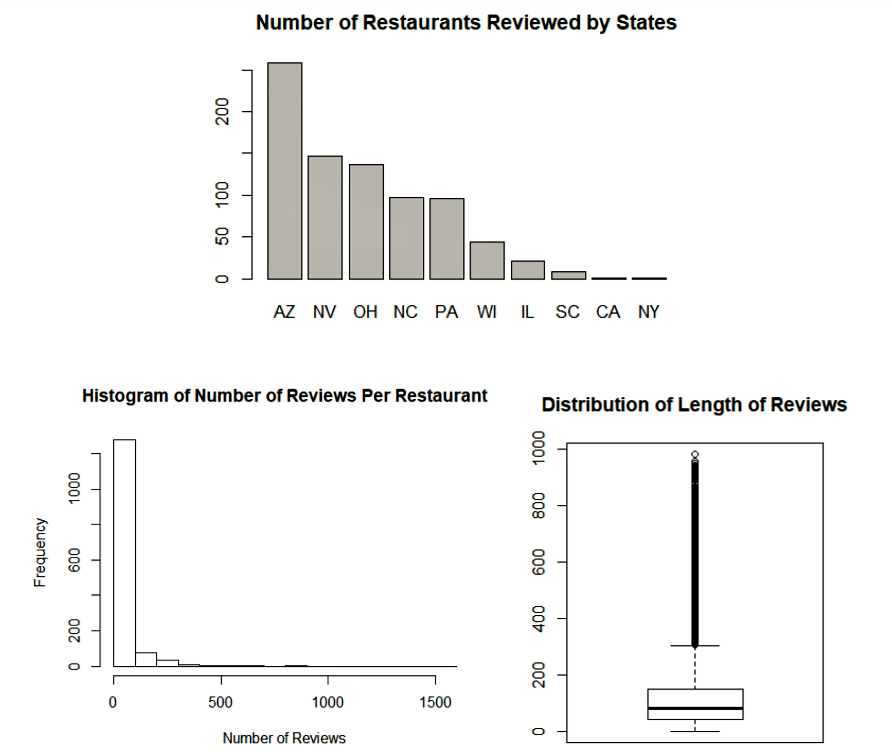
\includegraphics{figure/EDA_combined.png}
\caption{\label{fig:EDA}Plots illustrating EDA insights on reviews and
restaurants}
\end{figure}
\begin{figure}[htbp]
\centering
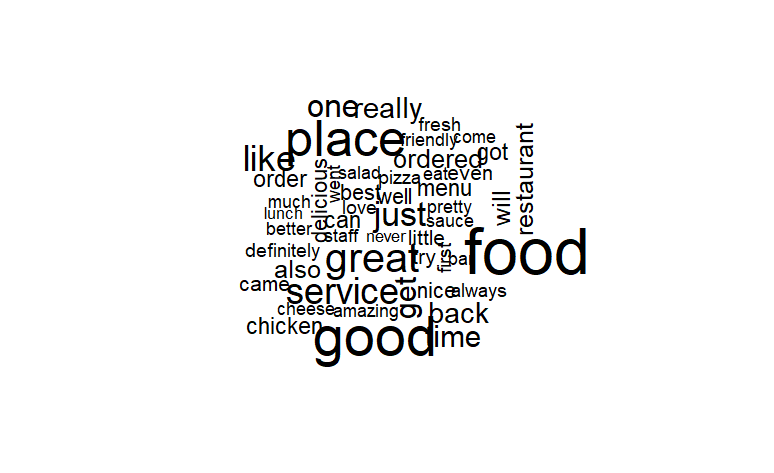
\includegraphics{figure/raw_wordcloud.png}
\caption{\label{fig:wordcloud}Word cloud of 50 most frequent words in corpus
(pre-stemming)}
\end{figure}
\section{N-Gramming}\label{n-gramming-1}

With the n-gramming model with hybrid cutoff thresholds detailed in the
Methodology section, 2148 bigrams and 406 trigrams or larger n-grams
were identified. Below is a table of the top and most representative
n-grams identified in our corpus of Yelp restaurant reviews.
\begin{longtable}[]{@{}ccc@{}}
\caption{\label{tab:bigram} Top Context-Specific Bigrams and
Trigrams}\tabularnewline
\toprule
\begin{minipage}[b]{0.31\columnwidth}\centering\strut
n-grams\strut
\end{minipage} & \begin{minipage}[b]{0.44\columnwidth}\centering\strut
Counts\strut
\end{minipage} & \begin{minipage}[b]{0.17\columnwidth}\centering\strut
p-value\strut
\end{minipage}\tabularnewline
\midrule
\endfirsthead
\toprule
\begin{minipage}[b]{0.31\columnwidth}\centering\strut
n-grams\strut
\end{minipage} & \begin{minipage}[b]{0.44\columnwidth}\centering\strut
Counts\strut
\end{minipage} & \begin{minipage}[b]{0.17\columnwidth}\centering\strut
p-value\strut
\end{minipage}\tabularnewline
\midrule
\endhead
\begin{minipage}[t]{0.31\columnwidth}\centering\strut
go\_back\strut
\end{minipage} & \begin{minipage}[t]{0.44\columnwidth}\centering\strut
3936\strut
\end{minipage} & \begin{minipage}[t]{0.17\columnwidth}\centering\strut
0.000000e+00\strut
\end{minipage}\tabularnewline
\begin{minipage}[t]{0.31\columnwidth}\centering\strut
high\_recommend\strut
\end{minipage} & \begin{minipage}[t]{0.44\columnwidth}\centering\strut
1814\strut
\end{minipage} & \begin{minipage}[t]{0.17\columnwidth}\centering\strut
0.000000e+00\strut
\end{minipage}\tabularnewline
\begin{minipage}[t]{0.31\columnwidth}\centering\strut
great\_food*\strut
\end{minipage} & \begin{minipage}[t]{0.44\columnwidth}\centering\strut
1723\strut
\end{minipage} & \begin{minipage}[t]{0.17\columnwidth}\centering\strut
1.060000e-75\strut
\end{minipage}\tabularnewline
\begin{minipage}[t]{0.31\columnwidth}\centering\strut
happi\_hour\strut
\end{minipage} & \begin{minipage}[t]{0.44\columnwidth}\centering\strut
1704\strut
\end{minipage} & \begin{minipage}[t]{0.17\columnwidth}\centering\strut
1.19e-75\strut
\end{minipage}\tabularnewline
\begin{minipage}[t]{0.31\columnwidth}\centering\strut
custom\_servic\strut
\end{minipage} & \begin{minipage}[t]{0.44\columnwidth}\centering\strut
1397\strut
\end{minipage} & \begin{minipage}[t]{0.17\columnwidth}\centering\strut
2.73e-26\strut
\end{minipage}\tabularnewline
\begin{minipage}[t]{0.31\columnwidth}\centering\strut
las\_vega\strut
\end{minipage} & \begin{minipage}[t]{0.44\columnwidth}\centering\strut
1057\strut
\end{minipage} & \begin{minipage}[t]{0.17\columnwidth}\centering\strut
7.60e-201\strut
\end{minipage}\tabularnewline
\begin{minipage}[t]{0.31\columnwidth}\centering\strut
white\_castl**\strut
\end{minipage} & \begin{minipage}[t]{0.44\columnwidth}\centering\strut
974\strut
\end{minipage} & \begin{minipage}[t]{0.17\columnwidth}\centering\strut
5.79e-152\strut
\end{minipage}\tabularnewline
\begin{minipage}[t]{0.31\columnwidth}\centering\strut
will\_definit.back\strut
\end{minipage} & \begin{minipage}[t]{0.44\columnwidth}\centering\strut
482\strut
\end{minipage} & \begin{minipage}[t]{0.17\columnwidth}\centering\strut
0.000000e+00\strut
\end{minipage}\tabularnewline
\begin{minipage}[t]{0.31\columnwidth}\centering\strut
mac\_n.chees\strut
\end{minipage} & \begin{minipage}[t]{0.44\columnwidth}\centering\strut
222\strut
\end{minipage} & \begin{minipage}[t]{0.17\columnwidth}\centering\strut
0.000000e+00\strut
\end{minipage}\tabularnewline
\begin{minipage}[t]{0.31\columnwidth}\centering\strut
food.pretti\_good*\strut
\end{minipage} & \begin{minipage}[t]{0.44\columnwidth}\centering\strut
166\strut
\end{minipage} & \begin{minipage}[t]{0.17\columnwidth}\centering\strut
1.270000e-121\strut
\end{minipage}\tabularnewline
\begin{minipage}[t]{0.31\columnwidth}\centering\strut
seat.right\_away\strut
\end{minipage} & \begin{minipage}[t]{0.44\columnwidth}\centering\strut
113\strut
\end{minipage} & \begin{minipage}[t]{0.17\columnwidth}\centering\strut
7.160000e-228\strut
\end{minipage}\tabularnewline
\begin{minipage}[t]{0.31\columnwidth}\centering\strut
matt\_big.breakfast***\strut
\end{minipage} & \begin{minipage}[t]{0.44\columnwidth}\centering\strut
101\strut
\end{minipage} & \begin{minipage}[t]{0.17\columnwidth}\centering\strut
2.550000e-296\strut
\end{minipage}\tabularnewline
\begin{minipage}[t]{0.31\columnwidth}\centering\strut
give\_place.star\strut
\end{minipage} & \begin{minipage}[t]{0.44\columnwidth}\centering\strut
99\strut
\end{minipage} & \begin{minipage}[t]{0.17\columnwidth}\centering\strut
2.430000e-184\strut
\end{minipage}\tabularnewline
\begin{minipage}[t]{0.31\columnwidth}\centering\strut
kung\_pao.chicken\strut
\end{minipage} & \begin{minipage}[t]{0.44\columnwidth}\centering\strut
54\strut
\end{minipage} & \begin{minipage}[t]{0.17\columnwidth}\centering\strut
8.850000e-119\strut
\end{minipage}\tabularnewline
\begin{minipage}[t]{0.31\columnwidth}\centering\strut
fast\_food.chain\strut
\end{minipage} & \begin{minipage}[t]{0.44\columnwidth}\centering\strut
40\strut
\end{minipage} & \begin{minipage}[t]{0.17\columnwidth}\centering\strut
1.24e-79\strut
\end{minipage}\tabularnewline
\bottomrule
\end{longtable}
Notes on the Bigram Trigram table:\\
1. (*) Similar bigrams including
\emph{``good/great\_food/servic/place''} are also common with
significant p-values. Same as in the case of trigrams:
\emph{``food/servic.pretti/realli/super\_good/great''}.\\
2. (**) Refers to ``White Castle'', a fast-food chain in Midwestern and
Mid-Atlantic regions of the United States. As previously mentioned, the
high occurrence of this bigram is likely due to the state distribution
of the reviewed restaurants in our corpus.\\
3. (***) Name of a reviewed restaurant in Phoenix, AZ. Same as above,
the high occurrence and significance of p-value of this trigram is also
related to our corpus-specific restaurant distributions. But in both
cases, identifying the word sequence as one token would carry the right
meaningful information and thus beneficial for the analysis.

\section{Topic Extraction}\label{topic-extraction-1}

Regardless of the method used for identifying common topics in the
corpus, we may first set our intuitive expectations for the output as a
qualitative sanity check. Given that our corpus is a set of reviews on
restaurants, commonly reviewed aspects may include food (eg. taste,
portion, price), service (eg. timeliness, friendliness), ambience (eg.
noise level, suitable occasion), location, etc.. We will see if these
targeted aspects can be recovered automatically.

\subsection{LDA}\label{lda}

With number of topics manually set at 5 and Gibbs sampling control slots
set at default level (again, a future step could be optimizing these
parameters automatically), the topics identified by the LDA model from
our corpus along with top words/tokens in each topic is listed below:

\label{tab:LDA-result}LDA topics and associated top terms (entire corpus,
stemmed)

Topic 1

Topic 2

Topic 3

Topic 4

Topic 5

place

burger

just

restaur

tabl

locat

chicken

pizza

delici

order

sandwich

sauc

get

meal

ask

day

flavor

eat

salad

us

bar

fri

like

menu

said

alway

order

place

amaz

server

beer

tast

think

dinner

servic

love

good

im

steak

time

friend

meat

price

great

went

great

like

realli

bread

one

The above topics are approximately about restaurant - location and type
(Topic 1), food - variety and taste (Topic 2), food - type and price
(Topic 3), food - taste and variety (Topic 4), service (Topic 5). While
Topic 2 and Topic 4 seems to focus on approximately the same aspects,
the former is more about fast-food type of food while the latter seems
to be about fine dining.

I have also experimented with running LDA with sub-corpus of each
category listed on Yelp (i.e.~by cuisine type), and besides showing more
category-specific top terms such as ``taco'', ``salsa'', and
``horchata'' in the food topic for the sub-corpus of Mexican
restaurants, the segmented corpus did not result in significant
improvements in the distinction of topics but rather had worse
performance possibly due to less documents in sub-corpus. While
segmentation of corpus proves to not be of much help when extracting
common topics, it may be helpful later in the step of sentiment
aggregation especially we decide to use top terms associated with
targeted topics (food, service, ambience, location etc.) as the
anchor/center for finding and aggregating sentiment polarity.

\chapter{Discussion}\label{discussion}

Your paper should be an evolving report on the project in all aspects
developed so far, in the form of a draft scientific paper. It must be
written in RMarkdown or LaTeX with figures included.

Make sure all figures have font sizes and line widths set so that the
final pdf versions are properly legible. Presentation (including
correctness of mathematical equations, graphics, tables, citations and
bibligraphy, as well as prose) should be pristine.

All details of developments of models, code and examples/analyses must
be clearly described -- sufficient to that a knowledgeable reader will
be able to follow the logic and replicate the analysis.

By the end of the first (Fall) semester, you need to develop a readable
interim report. In the second (Spring) semester your task is to evolve
this paper into a complete write-up of your work, as if intending to
consider submitting to a scientific journal.

However primitive the content may seem to be at the start, start
writing.

A fairly standard outline is as follows:
\begin{itemize}
\tightlist
\item
  \textbf{Title}
\item
  \textbf{Abstract}
\item
  \textbf{Chapter 1. Introduction} (setting, problem description,
  citations, etc.)
\item
  \textbf{Chapter 2. Literature review}
\item
  \textbf{A Next Chapter:} Some papers have one or two chapters, some
  papers have several. Keep chapters relatively short: Each section
  should have one focus. For example,
  \begin{itemize}
  \tightlist
  \item
    \textbf{Chapter 3. New Statistical Models} (theory, ideas)
  \item
    \textbf{Chapter 4. Some Computational Issues}
  \item
    \textbf{Chapter 5. Simulated Data} (evaluation of models)
  \item
    \textbf{Chapter 6. Application} (real motivating problem and data)
  \item
    \ldots{}
  \end{itemize}
\item
  \textbf{Chapter X. Conclusion} (what was done, what was learned, what
  was good/bad, where research might or could go next)
\item
  \textbf{Appendix} (maybe some extra math, details of code)
\item
  \textbf{Bibliography} (use bibtex, per the example bib files)
\end{itemize}
\chapter*{Conclusion}\label{conclusion}
\addcontentsline{toc}{chapter}{Conclusion}

If we don't want Conclusion to have a chapter number next to it, we can
add the \texttt{\{-\}} attribute.

\textbf{More info}

And here's some other random info: the first paragraph after a chapter
title or section head \emph{shouldn't be} indented, because indents are
to tell the reader that you're starting a new paragraph. Since that's
obvious after a chapter or section title, proper typesetting doesn't add
an indent there.

\appendix

\chapter{The First Appendix}\label{the-first-appendix}

This first appendix includes all of the R chunks of code that were
hidden throughout the document (using the \texttt{include\ =\ FALSE}
chunk tag) to help with readibility and/or setup.

\textbf{In the main Rmd file}
\begin{Shaded}
\begin{Highlighting}[]
\CommentTok{# This chunk ensures that the thesisdowndss package is}
\CommentTok{# installed and loaded. This thesisdowndss package includes}
\CommentTok{# the template files for the thesis.}
\NormalTok{if(!}\KeywordTok{require}\NormalTok{(devtools))}
  \KeywordTok{install.packages}\NormalTok{(}\StringTok{"devtools"}\NormalTok{, }\DataTypeTok{repos =} \StringTok{"http://cran.rstudio.com"}\NormalTok{)}
\NormalTok{if(!}\KeywordTok{require}\NormalTok{(thesisdowndss))}
  \NormalTok{devtools::}\KeywordTok{install_github}\NormalTok{(}\StringTok{"mine-cetinkaya-rundel/thesisdowndss"}\NormalTok{)}
\KeywordTok{library}\NormalTok{(thesisdowndss)}
\end{Highlighting}
\end{Shaded}
\textbf{In Chapter \ref{ref-labels}:}
\begin{Shaded}
\begin{Highlighting}[]
\CommentTok{# This chunk ensures that the thesisdowndss package is}
\CommentTok{# installed and loaded. This thesisdowndss package includes}
\CommentTok{# the template files for the thesis and also two functions}
\CommentTok{# used for labeling and referencing}
\NormalTok{if(!}\KeywordTok{require}\NormalTok{(devtools))}
  \KeywordTok{install.packages}\NormalTok{(}\StringTok{"devtools"}\NormalTok{, }\DataTypeTok{repos =} \StringTok{"http://cran.rstudio.com"}\NormalTok{)}
\NormalTok{if(!}\KeywordTok{require}\NormalTok{(dplyr))}
    \KeywordTok{install.packages}\NormalTok{(}\StringTok{"dplyr"}\NormalTok{, }\DataTypeTok{repos =} \StringTok{"http://cran.rstudio.com"}\NormalTok{)}
\NormalTok{if(!}\KeywordTok{require}\NormalTok{(ggplot2))}
    \KeywordTok{install.packages}\NormalTok{(}\StringTok{"ggplot2"}\NormalTok{, }\DataTypeTok{repos =} \StringTok{"http://cran.rstudio.com"}\NormalTok{)}
\NormalTok{if(!}\KeywordTok{require}\NormalTok{(ggplot2))}
    \KeywordTok{install.packages}\NormalTok{(}\StringTok{"bookdown"}\NormalTok{, }\DataTypeTok{repos =} \StringTok{"http://cran.rstudio.com"}\NormalTok{)}
\NormalTok{if(!}\KeywordTok{require}\NormalTok{(thesisdowndss))\{}
  \KeywordTok{library}\NormalTok{(devtools)}
  \NormalTok{devtools::}\KeywordTok{install_github}\NormalTok{(}\StringTok{"mine-cetinkaya-rundel/thesisdowndss"}\NormalTok{)}
  \NormalTok{\}}
\KeywordTok{library}\NormalTok{(thesisdowndss)}
\CommentTok{# flights <- read.csv("data/flights.csv")}
\KeywordTok{library}\NormalTok{(topicmodels)}
\NormalTok{lda <-}\StringTok{ }\KeywordTok{readRDS}\NormalTok{(}\StringTok{"data/LDA_all_ngrammed.rds"}\NormalTok{)}
\end{Highlighting}
\end{Shaded}
\chapter{The Second Appendix, for
Fun}\label{the-second-appendix-for-fun}

\backmatter

\chapter*{References}\label{references}
\addcontentsline{toc}{chapter}{References}

\markboth{References}{References}

\noindent

\setlength{\parindent}{-0.20in} \setlength{\leftskip}{0.20in}
\setlength{\parskip}{8pt}

\hypertarget{refs}{}
\hypertarget{ref-angel2000}{}
Angel, Edward. 2000. \emph{Interactive Computer Graphics : A Top-down
Approach with Opengl}. Boston, MA: Addison Wesley Longman.

\hypertarget{ref-angel2001}{}
---------. 2001a. \emph{Batch-File Computer Graphics : A Bottom-up
Approach with Quicktime}. Boston, MA: Wesley Addison Longman.

\hypertarget{ref-angel2002a}{}
---------. 2001b. \emph{Test Second Book by Angel}. Boston, MA: Wesley
Addison Longman.


% Index?

\end{document}
